At the core of every synthesizer is the ability to generate forensic
artifacts as part of a larger scenario; this chapter addresses the AKF
modules responsible for automating artifact generation, depicted in
\autoref{fig:actions-simple} below. The detailed diagrams for these
modules are part of \autoref{appendix-a}, depicted in
\autoref{fig:architecture-full-b} and \autoref{fig:architecture-full-d}.

\begin{figure}[h]
\centering
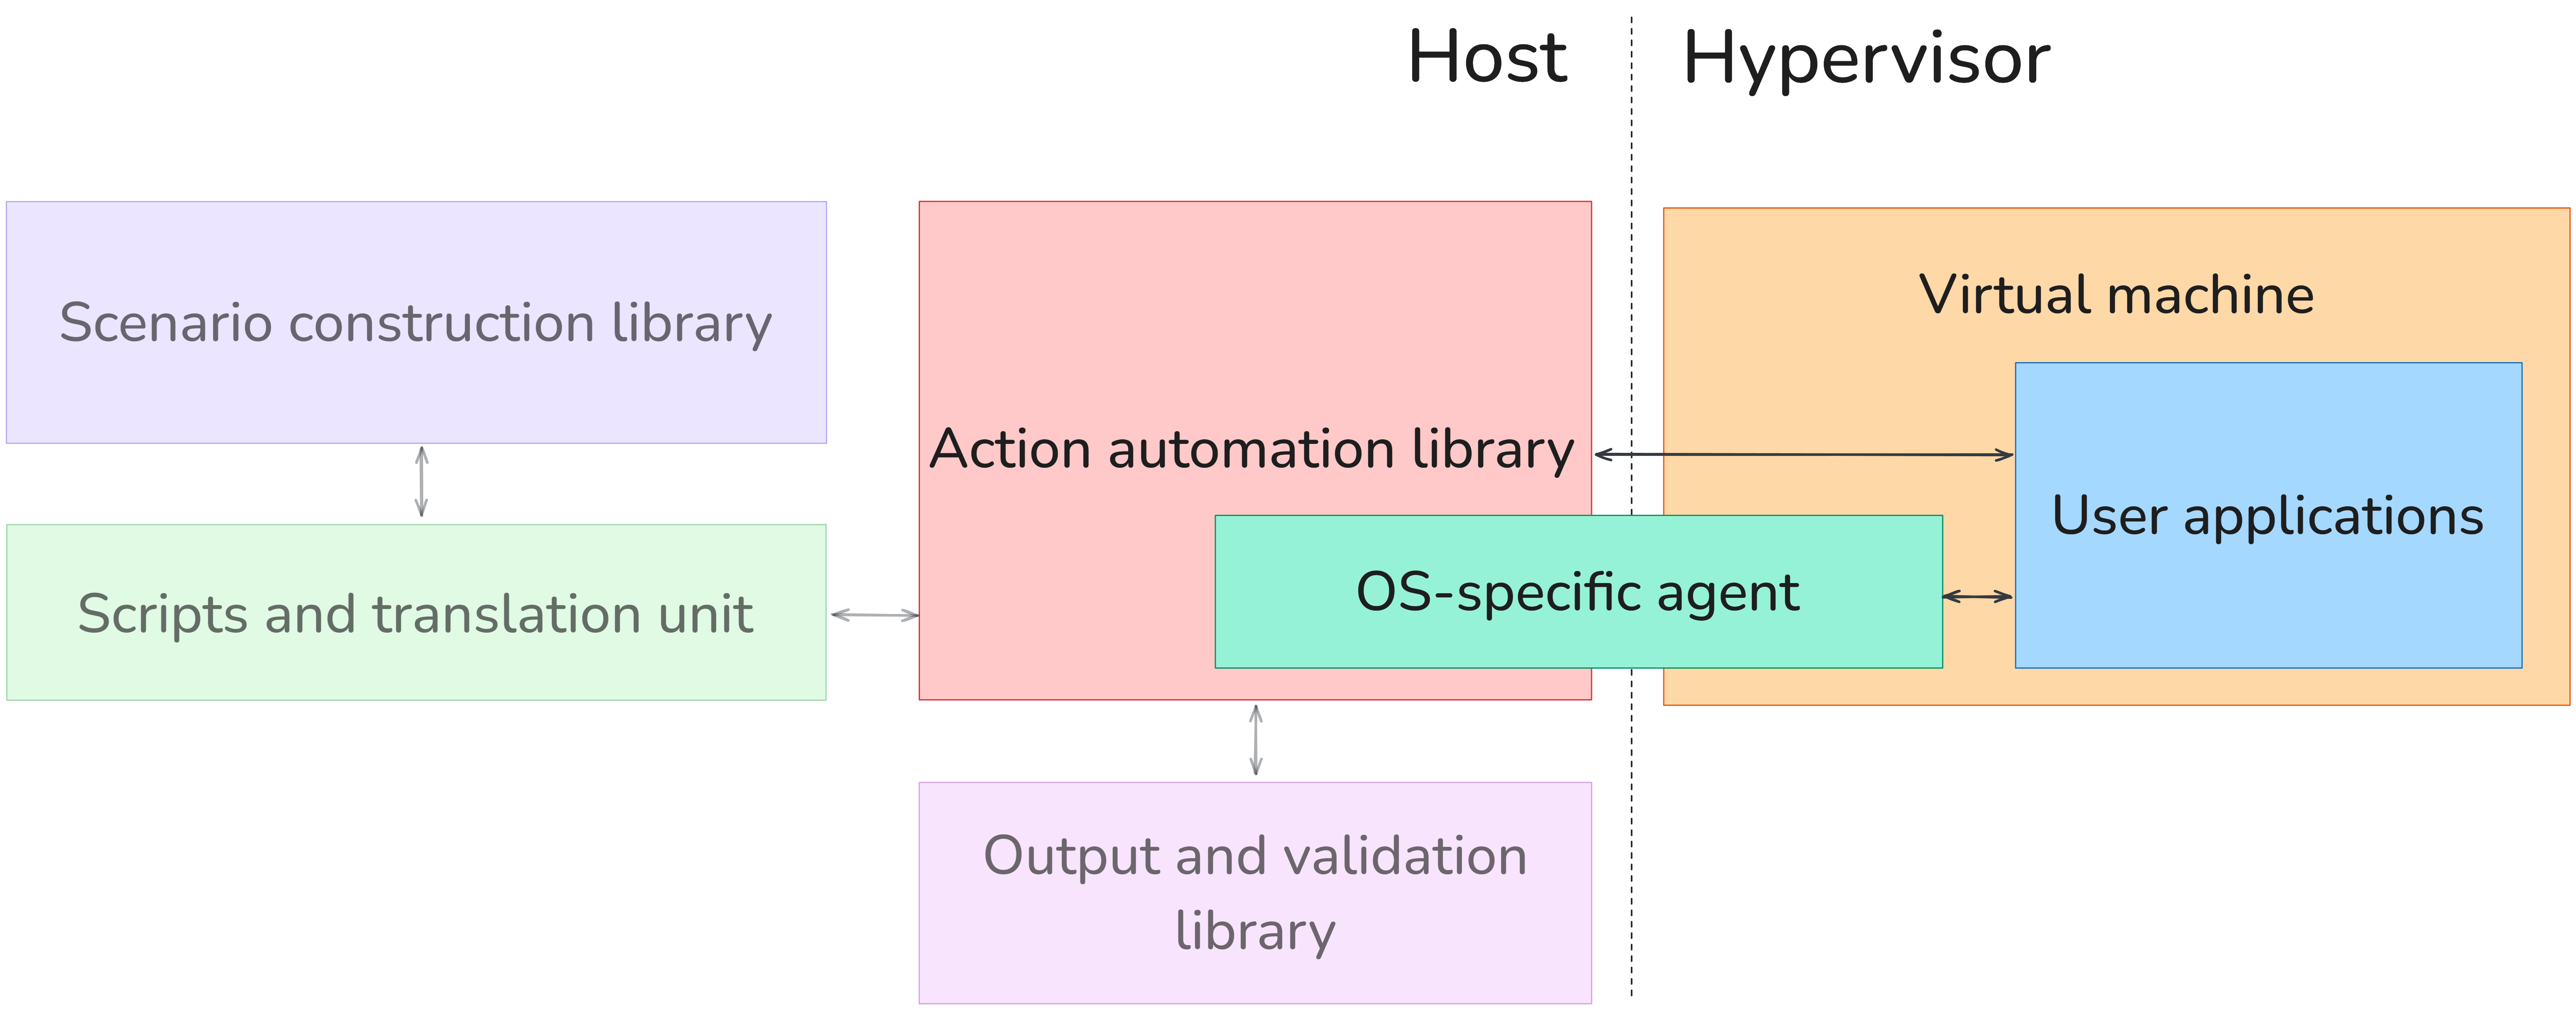
\includegraphics[width=1\linewidth]{actions-simple.png}
\caption{Simplified AKF architecture diagram for scenario construction
modules}\label{fig:actions-simple}
\end{figure}

Each of the synthesizers described in \autoref{analysis-of-existing-synthesizers} takes one of three
approaches to artifact generation, as partly described by Scanlon et al.
\cite{scanlonEviPlantEfficientDigital2017}:

\begin{itemize}
\tightlist
\item
  \textbf{Physical}: No virtualization of software or hardware ever
  occurs; data is written directly to the target medium, such as a disk
  image or virtual hard drive.
\item
  \textbf{Agentless logical}: The synthesizer interacts with a live VM
  to generate artifacts. Interaction is achieved without the need for
  custom software to be installed on the VM; instead, actions are
  achieved using the hypervisor itself or a remote management tool
  native to the virtualized operating system.
\item
  \textbf{Agent-based logical}: The synthesizer interacts with a
  dedicated client, or agent, on a live VM to carry out actions. The VM
  must have the agent installed before any interaction can occur.
\end{itemize}

These three approaches are not mutually exclusive within a single
synthesizer, though many prior synthesizers have used only one approach
to generate artifacts. \autoref{tbl:prior-techniques} below denotes the
approaches used by each of the synthesizers previously discussed. Where
source code is unavailable, a best effort was made to identify the
approach used by a particular synthesizer based on its published paper,
if one exists; otherwise, the entire row contains question marks.


{
\small % 10pt font
\setstretch{1} % Single spacing
\begin{longtable}[]{@{}
  >{\raggedright\arraybackslash}p{(\linewidth - 6\tabcolsep) * \real{0.2}}
  >{\raggedright\arraybackslash}p{(\linewidth - 6\tabcolsep) * \real{0.2666}}
  >{\raggedright\arraybackslash}p{(\linewidth - 6\tabcolsep) * \real{0.2666}}
  >{\raggedright\arraybackslash}p{(\linewidth - 6\tabcolsep) * \real{0.2666}}
@{}}
\caption{Summary of artifact generation techniques in prior synthesizers}\label{tbl:prior-techniques} \\
\toprule\noalign{}
\begin{minipage}[b]{\linewidth}\raggedright
Synthesizer
\end{minipage} & \begin{minipage}[b]{\linewidth}\raggedright
Physical
\end{minipage} & \begin{minipage}[b]{\linewidth}\raggedright
Agentless
\end{minipage} & \begin{minipage}[b]{\linewidth}\raggedright
Agent-based
\end{minipage} \\
\midrule\noalign{}
\endhead
\bottomrule\noalign{}
\endlastfoot
\textbf{FALCON} \cite{adelsteinAutomaticallyCreatingRealistic2005},
2005 & ? & ? & ? \\
\textbf{CYDEST} \cite{bruecknerAutomatedComputerForensics2008}, 2008
& ? & ? & ? \\
\textbf{Forensig2}
\cite{mochForensicImageGenerator2009,mochEvaluatingForensicImage2012},
2009 & Yes (filesystem mounting; filesystem-independent editing) & Yes
(over SSH only) & No \\
\textbf{D-FET} \cite{williamCloudbasedDigitalForensics2011}, 2011 &
Yes (filesystem mounting; filesystem-independent editing) & No & No \\
\textbf{SFX} \cite{russellForensicImageDescription2012}, 2012 & Yes
(filesystem mounting) & No & No \\
\textbf{Yannikos et al.} \cite{yannikosDataCorporaDigital2014}, 2014
& ? & ? & ? \\
\textbf{ForGeOSI} \cite{maxfraggMaxfraggForGeOSI2023}, 2014 & No &
Yes (hypervisor interfaces) & No \\
\textbf{ForGe} \cite{vistiAutomaticCreationComputer2015}, 2015 & Yes
(filesystem-aware editing) & No & No \\
\textbf{ForGen} \cite{jjk422Jjk422ForGen2019}, 2016 & No & No &
No \\
\textbf{EviPlant} \cite{scanlonEviPlantEfficientDigital2017}, 2017 &
Yes (filesystem-independent editing) & No & Yes (unknown mechanism) \\
\textbf{VMPOP} \cite{parkTREDEVMPOPCultivating2018}, 2018 & No & Yes
(hypervisor interfaces) & No \\
\textbf{hystck} \cite{gobelNovelApproachGenerating2020}, 2020 & No &
No & Yes (Python agent) \\
\textbf{TraceGen} \cite{duTraceGenUserActivity2021}, 2021 & No & No
& Yes (unknown mechanism) \\
\textbf{ForTrace} \cite{gobelForTraceHolisticForensic2022}, 2022 &
No & No & Yes (Python agent) \\
\end{longtable}
}


There are advantages and disadvantages to each approach, in addition to
requiring distinct implementation techniques for each. The remainder of
this chapter analyzes each of these three approaches in greater detail,
describing the implementation details of prior synthesizers and
comparing them to those of AKF's.

More specifically, this chapter addresses the functionality of the
action automation library (\passthrough{\lstinline!akflib!}) to generate
artifacts by either interacting with a live virtual machine or by
directly editing disk images stored on the host. We explore how logical
artifacts are generated at a lower level using hypervisor APIs and an
OS-specific agent running on the virtual machine. We conclude by
describing the generation of physical artifacts through direct
filesystem and disk image editing.

\section{Agentless artifact
generation}\label{agentless-artifact-generation}

\textbf{Agentless artifact creation} describes one of two general
techniques. The first is emulating ``normal'' human interaction by
leveraging virtualized human interfaces -- such as the monitor,
keyboard, and mouse -- to directly manipulate a GUI-based operating
system. The second is using (remote) management utilities included with
the operating system, typically an interactive shell.

AKF allows users to perform agentless artifact creation through a
hypervisor-agnostic interface; a concrete implementation of this
interface using VirtualBox is provided. This VirtualBox-specific
functionality is derived mainly from ForGeOSI
\cite{maxfraggMaxfraggForGeOSI2023}, which uses the VirtualBox SDK
and a Python implementation of the VirtualBox COM API
\cite{larsonSethmlarsonVirtualboxpython2025} to carry out the vast
majority of its tasks. This was adapted in VMPOP
\cite{parkTREDEVMPOPCultivating2018}, which also introduced the
notion of a generic hypervisor interface that allows for synthesizer
routines to use arbitrary hypervisors so long as required functionality
is implemented.

Note that the use of hypervisor-specific guest software, such as
VirtualBox Guest Additions and VMWare Tools, is treated as an agentless
approach for this thesis. Although this inherently requires installing
``unusual'' software on the virtual machine, it is very distinct from
typical user software. In many cases, artifacts generated by hypervisor
guest software can be identified, isolated, and ignored.

Relevant AKF submodules for agentless generation are depicted as opaque
elements in \autoref{fig:action-agentless}.

\begin{figure}[h]
\centering
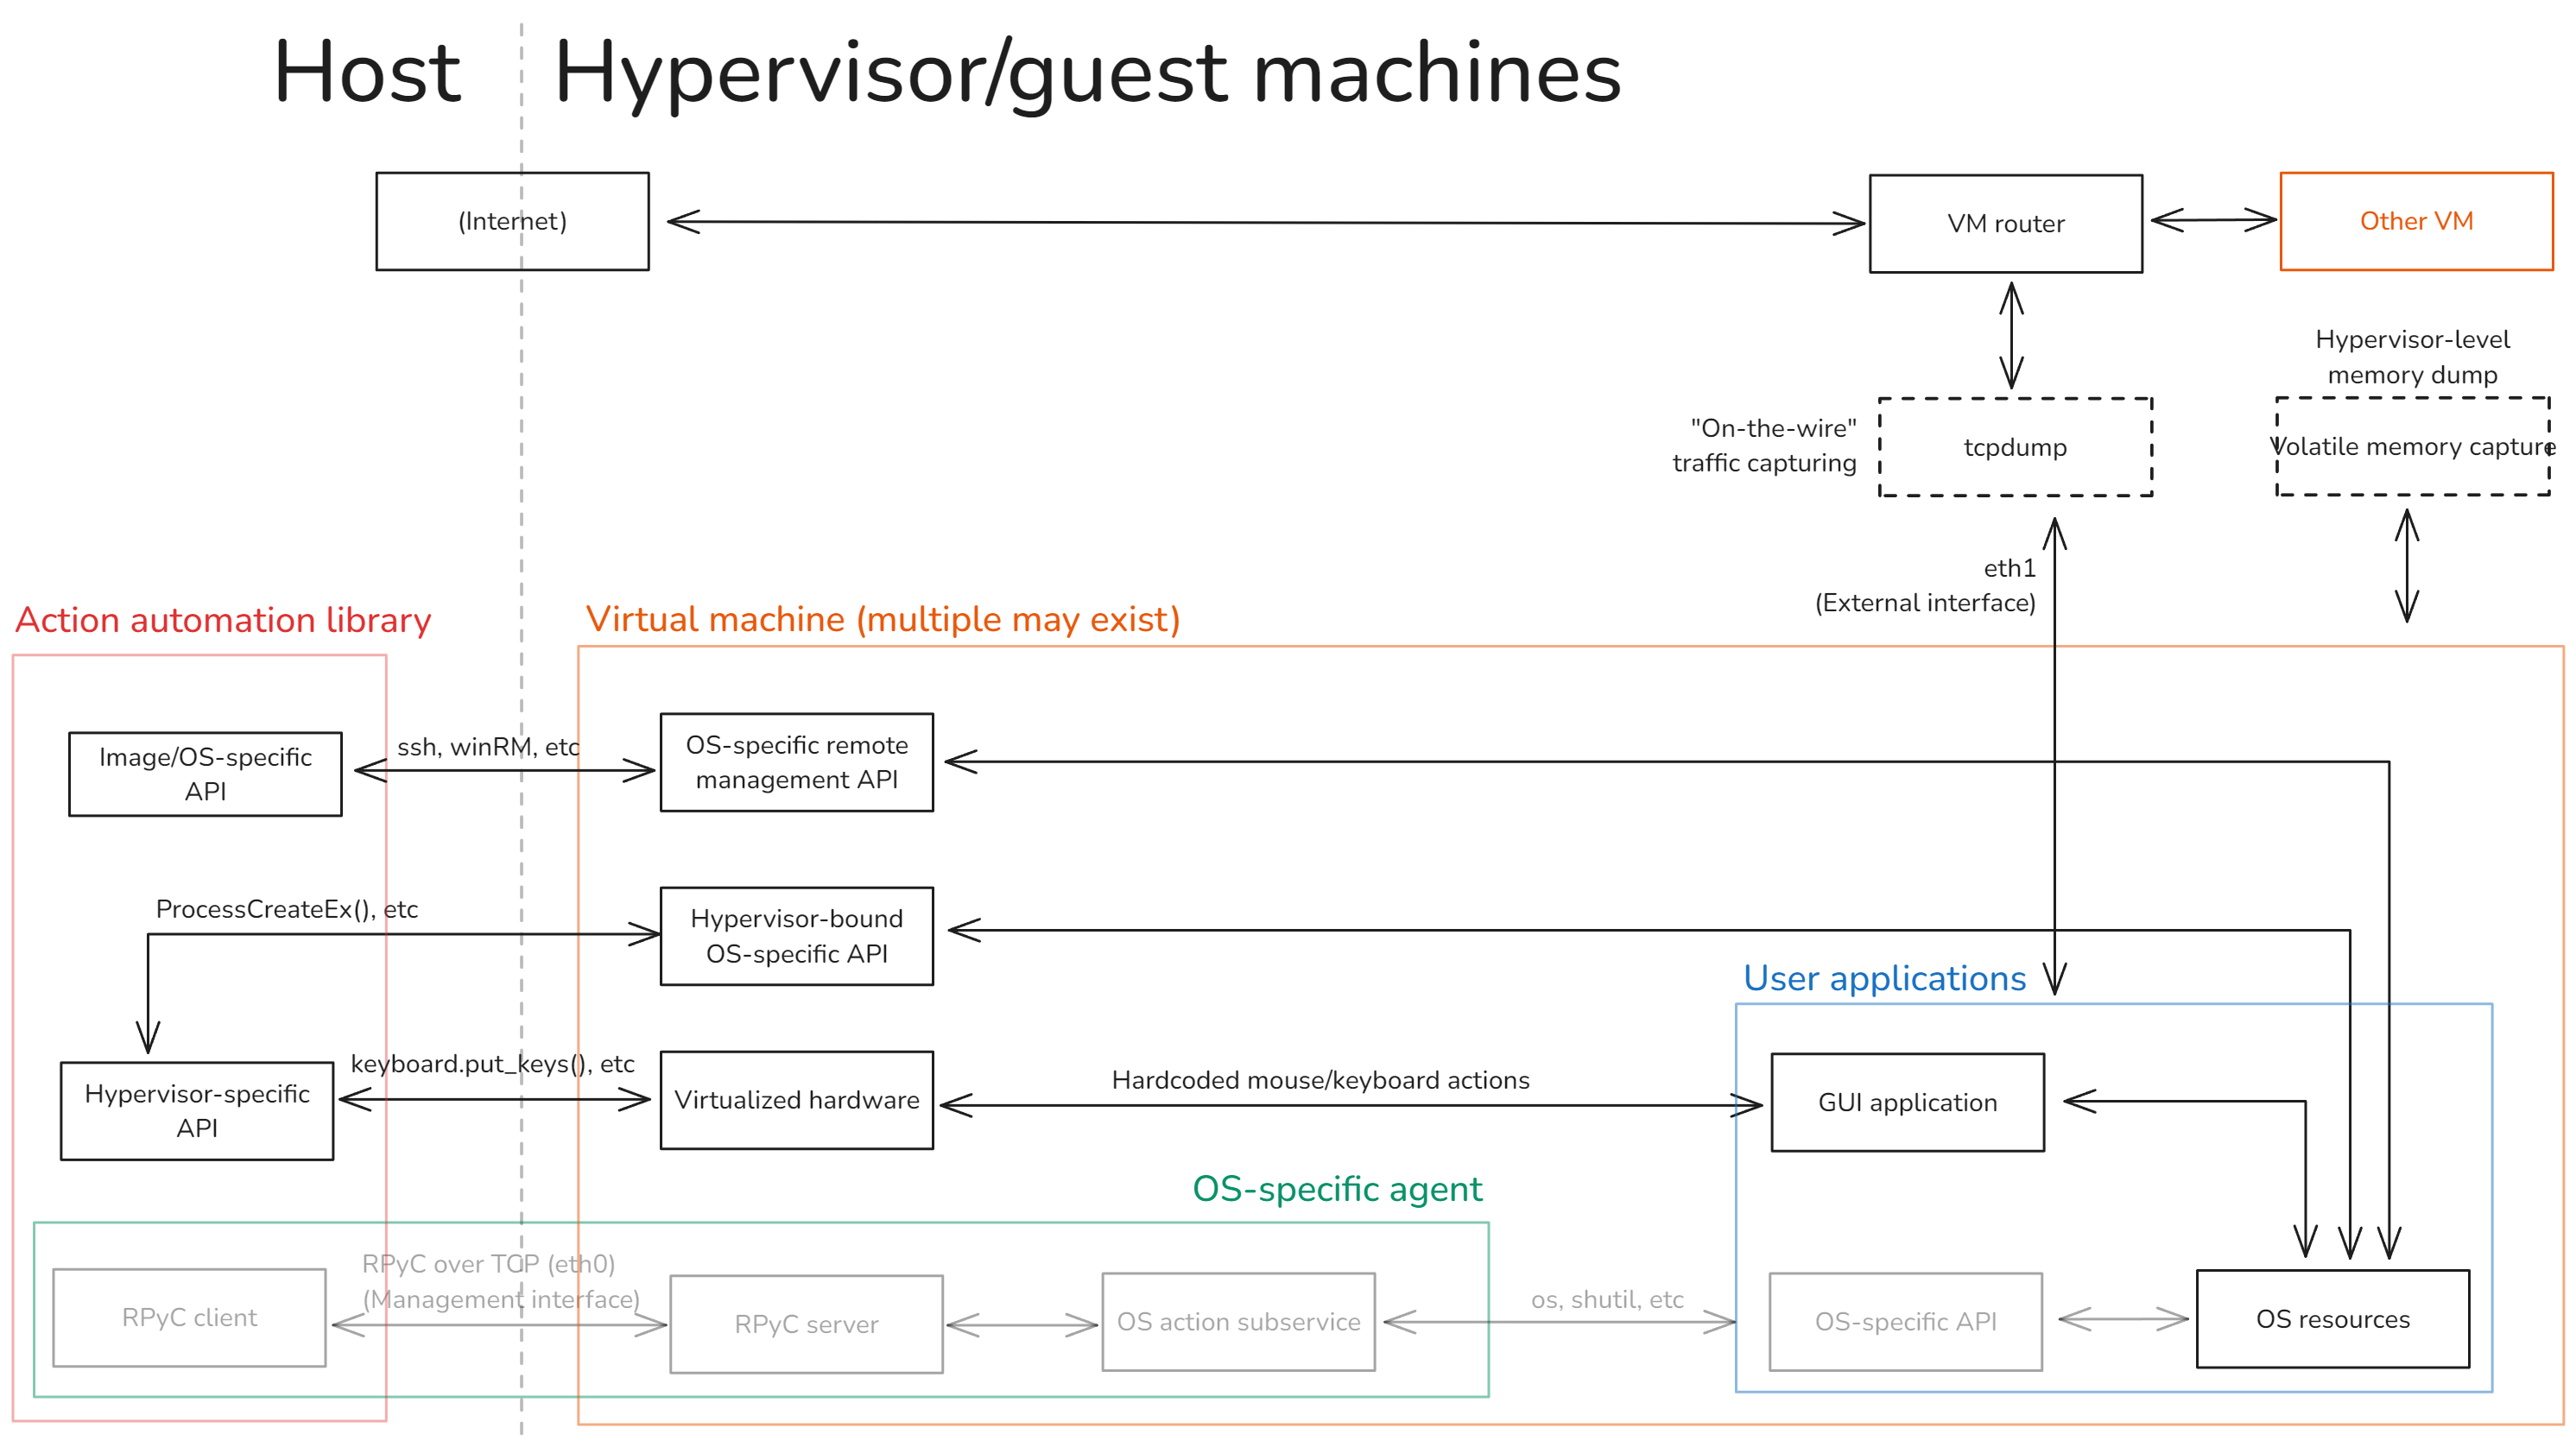
\includegraphics[width=1\linewidth]{action-agentless.png}
\caption{Abridged submodule diagram for agentless artifact
creation}\label{fig:action-agentless}
\end{figure}

\subsection{Human interfaces}\label{human-interfaces}

The use of human input devices -- the keyboard and mouse -- is the
primary approach taken by VMPOP \cite{parkTREDEVMPOPCultivating2018}
and ForGeOSI \cite{maxfraggMaxfraggForGeOSI2023} to generate
artifacts. For example, VMPOP uses a sequence of keyboard strokes to
focus and interact with UI elements, such as clearing User Account
Control dialogs on Windows or starting applications with Win+R. It
achieves this by making calls to the VirtualBox API, which issues
scancodes to the virtual machine.

This approach most accurately reflects how an actual human would
interact with a machine. As a result, this greatly reduces the
irrelevant data generated as a result of synthesizer operation. However,
this often leads to verbose scripts that are only capable of performing
very specific actions. The keyboard and mouse actions required to
fulfill a particular action can change significantly between versions of
the same application, versions of the same operating system, and varying
screen sizes. For example, VMPOP handles User Account Control (UAC)
prompts on machines prior to Windows 7 by sending an Alt+Tab keystroke
to the machine, clicking the mouse at the center of the screen to focus
the UAC prompt, and then sending Alt+C to accept the prompt. On machines
running Windows 7 or later, this is instead achieved by focusing the UAC
prompt with the mouse and then sending Alt+Y to accept the prompt.

Similarly, VMPOP interacts with browsers exclusively through the use of
keyboard shortcuts. VMPOP supports simple interactions with a small
number of websites, such as logging into Microsoft or Google accounts,
but is dependent on the form elements remaining the same over time. That
is, VMPOP does not inspect the contents of the current webpage to
perform actions; it cannot react to design changes. If the page has new
focusable elements, the same keystroke sequence may no longer achieve
the desired effects. This lack of runtime logic, which amounts to
operating a computer with the monitor off, leads to brittle scripts that
can be tedious to fix and update.

AKF's generic hypervisor interface provides functions for both mouse and
keyboard actions. While this is theoretically sufficient to emulate
nearly all actions that a human would normally perform with a mouse and
keyboard, the AKF agent (as described in \autoref{the-akf-agent}) also exposes a more flexible mouse
and keyboard automation API that is strongly preferred over the
VirtualBox interface. More generally, the AKF agent leverages automation
frameworks capable of runtime UI analysis, reducing the inflexibility of
application-specific scripts.

TraceGen \cite{duTraceGenUserActivity2021} notes that the ideal
future is to use computer vision and AI to automate user actions from
high-level prompts. Performing a Google search in a specific browser
would currently require a sequence of predefined keystrokes, assuming an
agentless approach is needed. Future advancements in LLMs may make it
possible to allow a machine to perform arbitrarily complex tasks on a
GUI-based operating system using natural language -- an approach that
can be integrated into AKF in the future, as addressed in \autoref{open-ended-automation-with-ai}.

\subsection{Management utilities}\label{management-utilities}

The alternative is to use existing management utilities which are native
to the virtualized operating system and are capable of carrying out
commands. This approach can also be divided into two categories: local
management utilities, such as Bash and PowerShell, and remote management
utilities, such as SSH servers and WinRM.

Local management utilities typically refer to scripting languages that
are available as part of the operating system and can be used to manage
most or all operating system resources. For example, PowerShell allows
users to modify registry keys, invoke applications, create users, and
more. Similarly, any standard Linux shell, such as Bash or Zsh, can be
used to install packages and run various command-line applications.
These shells can be invoked by either opening and focusing a terminal
window (for example, through the Win+R shortcut on Windows) or directly
executing scripts through hypervisor guest additions.

In particular, VMPOP \cite{parkTREDEVMPOPCultivating2018} makes
heavy use of local management utilities; it implements much of its
functionality through a collection of PowerShell and batch scripts. For
example, VMPOP allows users to focus a window by process ID, process
name, or window title. This is achieved by getting a PowerShell handle
to the process using \passthrough{\lstinline!Get-Process!}, using
\passthrough{\lstinline!Add-Type!} to add a local C\# function that is
capable of sending keyboard events through
\passthrough{\lstinline!user32.dll!}, and then holding the Alt key while
using \passthrough{\lstinline!AppActivate!} to focus the window and
bring it to the foreground. VMPOP leverages similar scripts for
launching and terminating processes by name, uninstalling programs,
creating a Windows restore point, and more.

Similarly, remote management utilities allow a remote device to invoke
local management utilities, typically over an SSH server or WinRM. In
most synthesizer architectures, remote management utilities require that
the host and guest machines can communicate with each other. This is
typically achieved through a NAT or host-only interface managed by the
hypervisor. This approach is taken by Forensig2
\cite{mochForensicImageGenerator2009}, which exclusively connects to
a running SSH server on a virtual machine to carry out user actions.

The use of remote management utilities to automate actions typically
undertaken by users is not uncommon, especially with the prevalence of
infrastructure as code solutions. For example, the open-source Ansible
framework simplifies the configuration of Windows and Linux devices to
simple, YAML-based files called ``playbooks.'' These playbooks contain a
sequence of tasks to perform, such as installing packages, managing
local user accounts, and running scripts, which are executed on multiple
remote machines in parallel. (Ansible's high-level scripting language is
the inspiration for AKF's declarative scripting language, described in
\autoref{declarative-usage}.)

It is worth noting that although this approach does not require
installing new software on the machine, most operating systems perform
some degree of logging when their management utilities are invoked. For
example, the \passthrough{\lstinline!sshd!} daemon logs connections
regardless of whether a NAT or host-only network interface is used. This
behavior may make it difficult to separate or remove logs unrelated to a
scenario. Similarly, the invocation of PowerShell scripts generates
event logs, which can be particularly noisy if Script Block Logging
(which logs the execution and content of all PowerShell scripts) is
enabled.

AKF inherits the capabilities of VMPOP, allowing users to leverage the
VirtualBox API and Guest Additions for various actions. For example,
users can mount shared directories and copy artifacts from the host to
the guest machine. However, AKF does not currently implement any
agentless OS- or application-specific functionality through this method;
many of the actions and artifacts previously generated through
OS-specific scripts in VMPOP \cite{parkTREDEVMPOPCultivating2018}
and other synthesizers can be implemented with greater flexibility
through the agent. How this flexibility is achieved, as well as why it
is the preferred method for implementing application-specific
functionality, is described in the following section.

\section{Agent-based artifact
generation}\label{agent-based-artifact-generation}

\textbf{Agent-based artifact creation} involves the use of a dedicated
executable on the VM that serves as an interface between the host
machine and the guest machine. This program runs commands natively on
the virtual machine on behalf of the host machine, accepting commands
over a dedicated network interface. This allows for greater flexibility
and more complex actions to be taken when compared to agentless
approaches. In particular, it allows application-specific functionality
to be implemented using existing automation frameworks such as Selenium
\cite{SeleniumHQSelenium2025}, Playwright
\cite{MicrosoftPlaywrightpython2025}, and PyAutoGUI
\cite{sweigartAsweigartPyautogui2025}.

It is worth noting that agent-based artifact creation often leads to the
generation of extraneous artifacts that would never be seen in a
real-world dataset. For example, agents often do not interact with
applications in the same way that a human would, possibly creating
additional artifacts that would not exist if a human had performed the
same actions. As a result, the synthesizer should document
synthesizer-related artifacts that can be ignored for educational and
testing purposes.

Relevant AKF submodules for agent-based generation are depicted as
opaque elements in \autoref{fig:action-agent}.

\begin{figure}[h]
\centering
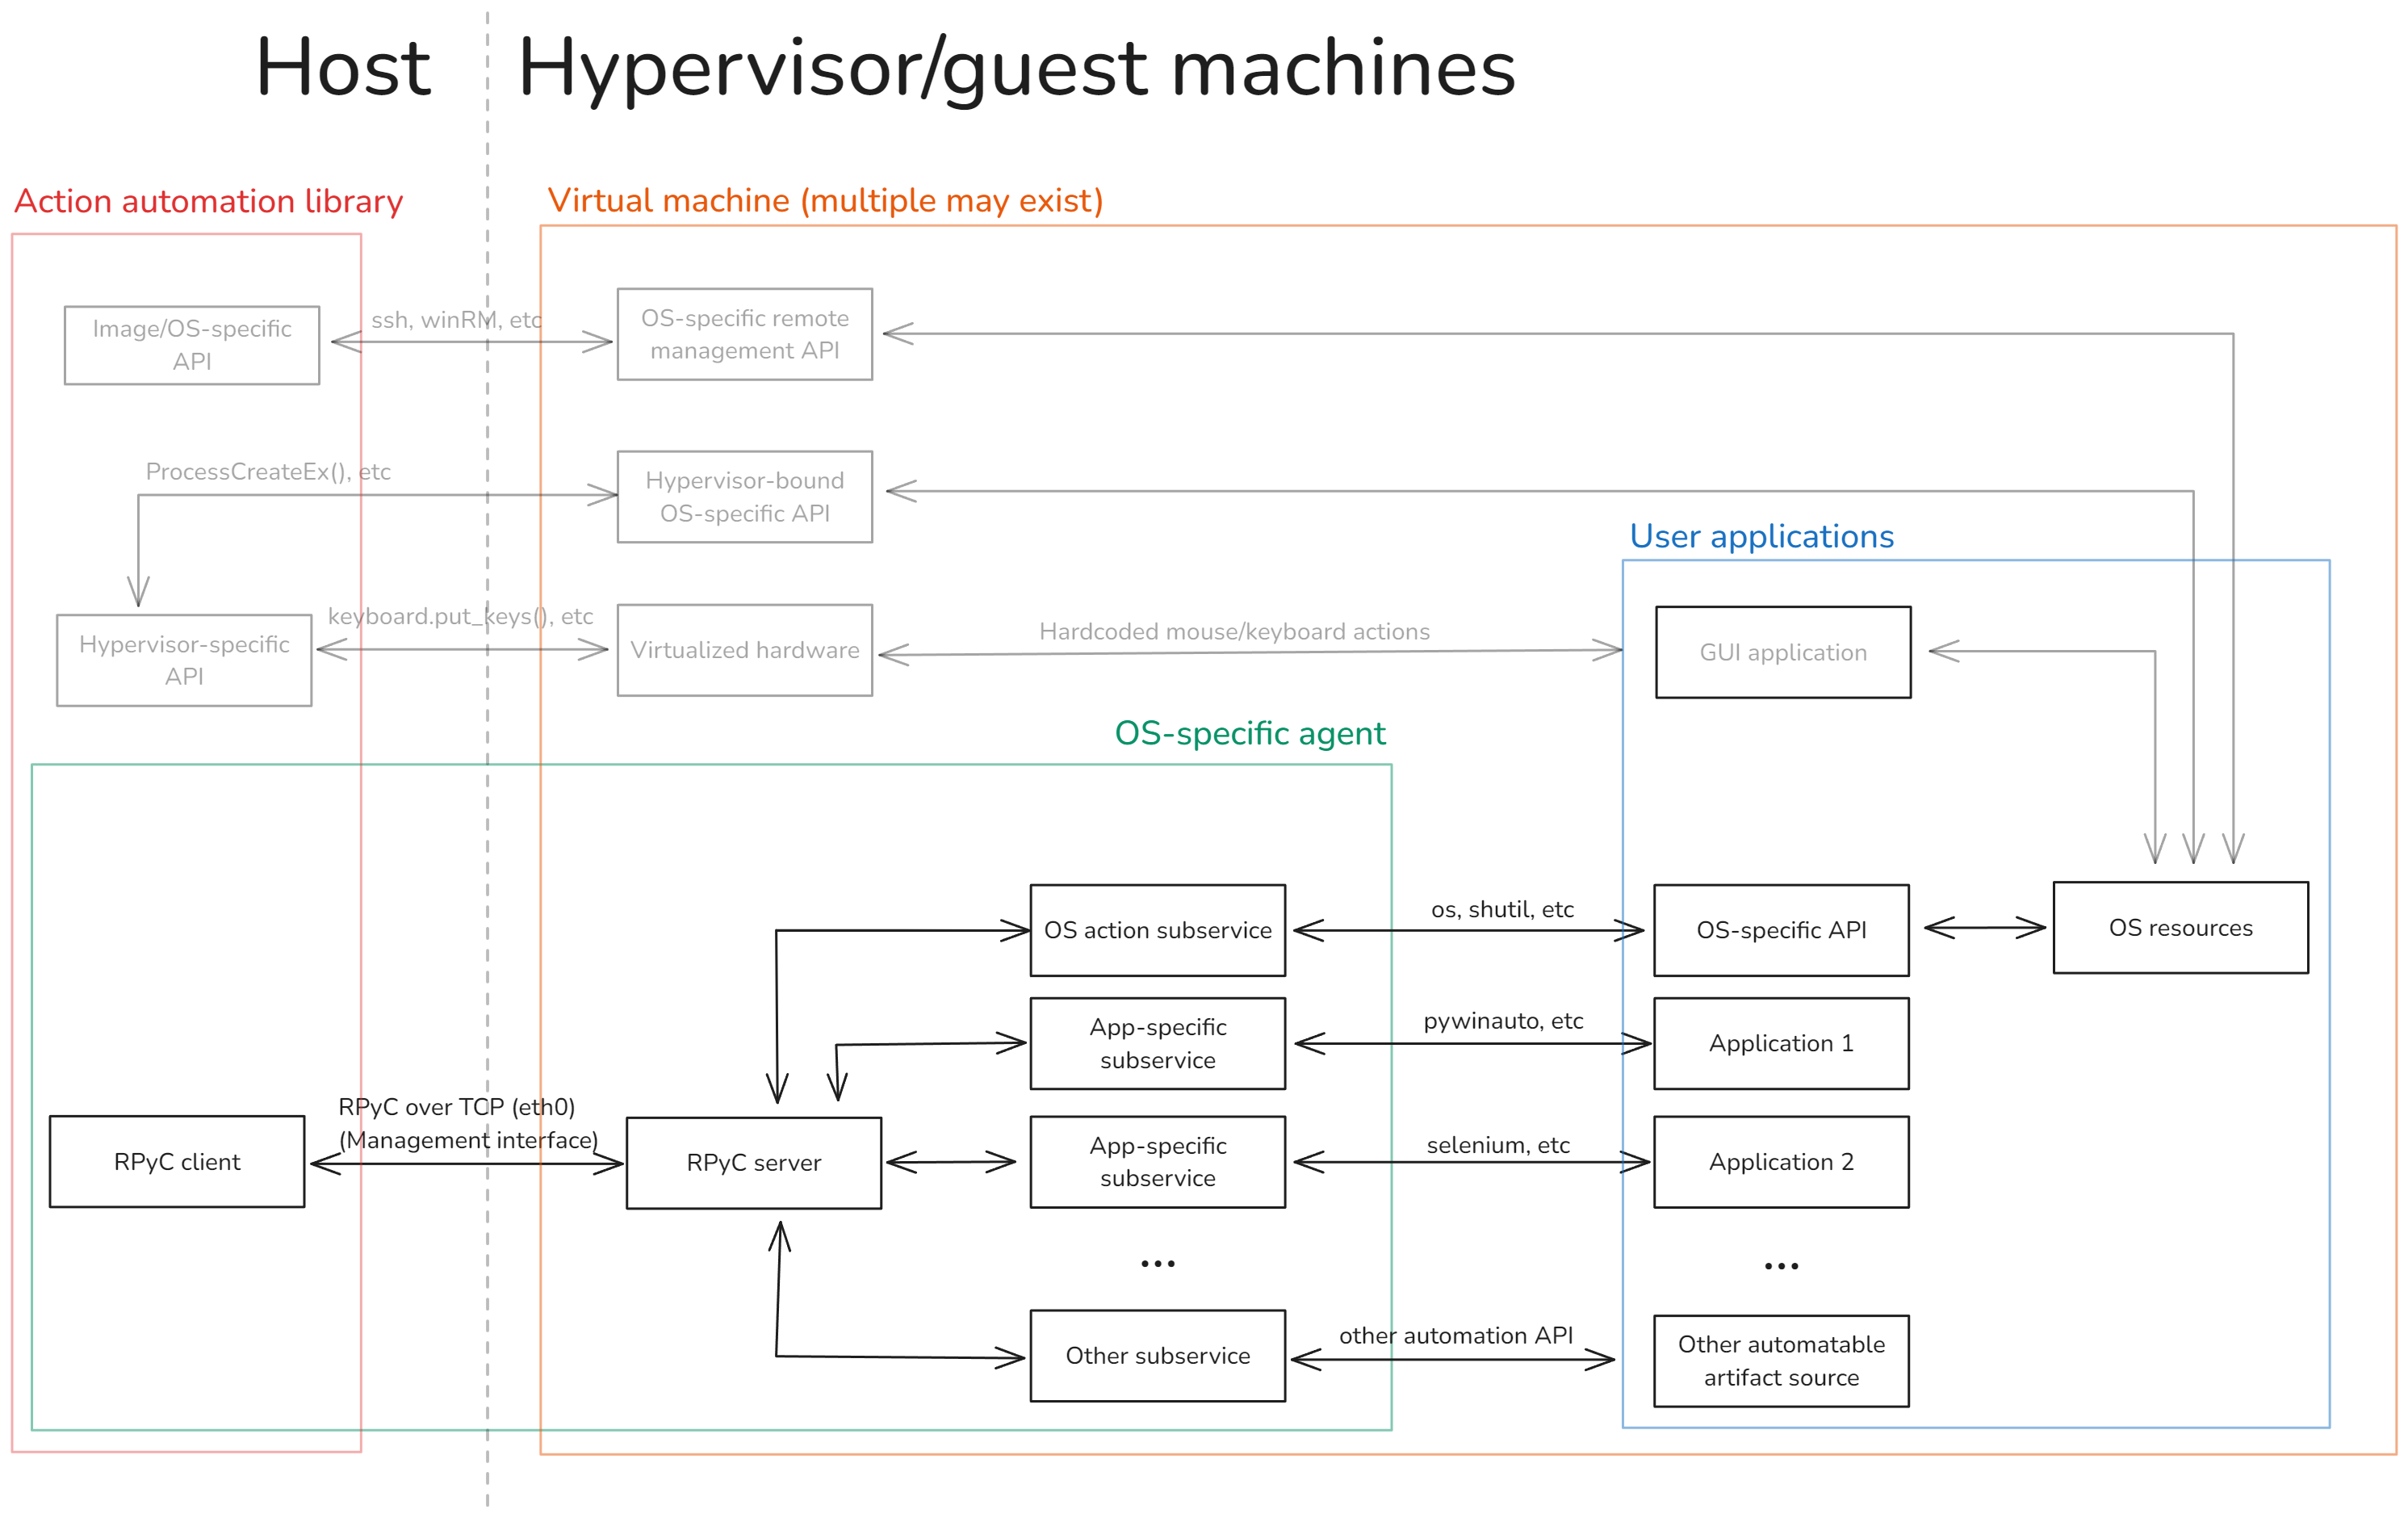
\includegraphics[width=1\linewidth]{action-agent.png}
\caption{Abridged submodule diagram for agent-based artifact
creation}\label{fig:action-agent}
\end{figure}

\subsection{Analysis of the ForTrace
agent}\label{analysis-of-the-fortrace-agent}

Agent-based artifact creation is the approach taken by hystck/ForTrace
\cite{gobelNovelApproachGenerating2020,gobelForTraceHolisticForensic2022},
which refers to its agent as an ``interaction manager.'' Because
ForTrace provides extensive agent functionality and is by far the most
mature synthesizer, AKF's agents borrow heavily from ForTrace's
approach. We briefly describe ForTrace's implementation of agents here,
with a more detailed analysis in \autoref{comparison-of-fortrace-and-akf-agents}.

ForTrace agents are simply an entire copy of the ForTrace codebase
copied over to the virtual machine -- that is, the ``agent'' and
``server'' share the same codebase but have different entry points and
use different parts of the ForTrace library. Communication between the
agent and the server occurs over a dedicated TCP socket using a simple
ASCII-based protocol; to execute commands, the server sends a
space-delimited string containing the application, function, and
arguments to run. Results are similarly returned by the agent as
structured ASCII messages. These messages are typically sent over a
dedicated ``management'' network interface to exclude them from network
captures for scenario-related activities.

Application-specific functionality for agents is organized into
individual files (Python modules), where each file includes a set of
commands or actions for a single application. These files contain both
server-side code (the logic for \emph{constructing} the ASCII message)
and agent-side code (the logic for \emph{interpreting} the message and
\emph{executing} the command) as a set of classes with a common prefix.
This common prefix is used to automatically discover the corresponding
agent-side code given a command issued by the server-side code.

Two key implementation details should be noted here. First, commands are
sent through a simple string-based protocol. This simplicity makes it
easy to debug issues arising from the protocol itself, but is relatively
inflexible as a result. In particular, it is challenging to send complex
Python objects as arguments or return values since these objects often
cannot be easily serialized to a string without loss of information. An
example relevant to AKF is passing Playwright browser objects, which
contain an internal state that is difficult to extract and reconstruct
using strings alone.

The second implementation detail involves the discovery and execution of
commands indicated by the protocol. ForTrace depends on Python's runtime
introspection to discover the correct modules and functions to call
based on the contents of a command string, importing these modules
during runtime. While this is a valid approach, it is more complex (and
difficult to follow) than the approach taken by AKF.

\subsection{The AKF agent}\label{the-akf-agent}

AKF borrows heavily from the Python agent-based approach of ForTrace but
improves upon its architecture in several respects. Details of low-level
improvements over ForTrace's agent architecture are described in more
detail in \autoref{comparison-of-fortrace-and-akf-agents}.

Perhaps the most significant difference is the use of RPyC, a library
for symmetric remote procedure calls, for agent communication
\cite{TomerfilibaorgRpyc2025}. Although the RPyC protocol is
symmetric, it is often used in typical client-server architectures to
allow clients to manipulate remote Python objects as if they were local
objects, as well as invoke remote (server) functions using local
(client) parameters. Delegating the serialization and deserialization of
complex objects to RPyC allows us to perform complex operations that
would have been difficult to implement with the simple string-based
protocol of ForTrace.

In ``new-style'' RPyC, this is achieved by running a \emph{service} on
the device where remote operations should be performed. Services expose
a set of functions and attributes that may be accessed remotely by an
RPyC client, listening on a specified TCP port for requests to access
these exposed elements. Clients access these functions and attributes by
name as if they were local objects; arguments passed to functions are
serialized and deserialized in the background, as are the results of
function calls and attribute accesses.

AKF's application-specific functionality is divided into individual RPyC
``subservices'' created on demand. The agent's main loop is itself a
``root'' RPyC service that is responsible for creating and destroying
these subservices upon request; all subservices are known to the root
service at initialization, eliminating the need to perform runtime
introspection to find application-specific modules. These subservices
are analogous to the agent-side code of individual ForTrace modules,
interpreting arguments and executing commands on behalf of the host
machine.

Clients are largely decoupled from the server's implementation of
individual services; they do not directly call or import RPyC service
functions. Instead, they call these functions by name from an untyped
connection object. Because the exposed functions (as well as their
signatures) and attributes cannot be inferred from the raw RPyC
connection alone, clients can implement a typed, concrete API to
construct RPyC calls. This abstracts the raw RPyC call (and the
existence of an RPyC connection) away from the user while also providing
the signatures of remote functions where there would otherwise be none.
This allows for type checking and autocompletion during development.
This is analogous to the client-side code of individual ForTrace
modules, constructing messages to the agent to execute commands.

Additionally, because the RPyC service and the API to that service are
separable, this allows us to break the API (which is used in scenario
scripts) and the agent logic itself into two separate libraries. This
has two advantages -- it makes it significantly easier to build and
generate standalone executables using tools like PyInstaller
\cite{PyinstallerPyinstaller2025}, and it may also slightly reduce
the size of the agent when installed onto the virtual machine. Unlike
ForTrace, whose agent installation process requires a batch script
installing various libraries and Python through the Chocolatey package
manager, AKF's agent only requires that a single executable is copied
over and configured to run on startup (in addition to setting relevant
firewall rules). The agent setup process can be further simplified using
Vagrant, which is described in \autoref{setup-and-basic-usage}.

From an implementation and usability perspective, this design provides
three significant improvements over the ForTrace protocol. First, the
routing of functions is wholly delegated to RPyC. Instead of manually
constructing a message with the function name and its associated
parameters (as strings) over the network, the process of serializing
parameters and routing them to the correct function call is abstracted
away by RPyC.

Second, this allows us to pass and return arbitrarily complex objects
(for which we do not have to manually write the serialization and
deserialization logic). When passing complex objects from the agent to
the server or vice versa, a reference to the object is sent over the
network and wrapped by a \emph{proxy object}, which behaves like the
original object \cite{TheoryOperationRPyC}. Importantly, it is
usually not necessary to distinguish between local and remote/proxy
objects of the same type when writing code, which eliminates the extra
complexity of using proxies.

Finally, the ability to interact with complex remote objects allows us
to significantly reduce the actual code written as part of the API
exposed to the host. For example, there is no need to implement a
wrapper for every method available as part of a Playwright page object;
instead, a reference to the Playwright object \emph{running on the
virtual machine} can be given to the host machine. Instead of writing
individual methods for opening pages, navigating to specific elements,
and so on, we can simply use the methods that already exist in the
Playwright object -- any local calls on the host's proxy object will
lead to remote outcomes on the host, as desired. This, of course, does
not preclude the ability to write convenience methods for more complex
actions requiring the Playwright object.

The list of subservices supported by the AKF Windows agent is described
in \autoref{tbl:akf-applications} below. Although only three subservices
are implemented, each subservice is an example of a distinct design
pattern that could be easily adapted to implement other
application-specific functionality.


{
\small % 10pt font
\setstretch{1} % Single spacing
\begin{longtable}[]{@{}
  >{\raggedright\arraybackslash}p{(\linewidth - 4\tabcolsep) * \real{0.2}}
  >{\raggedright\arraybackslash}p{(\linewidth - 4\tabcolsep) * \real{0.2}}
  >{\raggedright\arraybackslash}p{(\linewidth - 4\tabcolsep) * \real{0.6}}
@{}}
\caption{Implemented subservices for the AKF Windows agent}\label{tbl:akf-applications} \\
\toprule\noalign{}
\begin{minipage}[b]{\linewidth}\raggedright
Subservice
\end{minipage} & \begin{minipage}[b]{\linewidth}\raggedright
Dependencies
\end{minipage} & \begin{minipage}[b]{\linewidth}\raggedright
Features
\end{minipage} \\
\midrule\noalign{}
\endhead
\bottomrule\noalign{}
\endlastfoot
\passthrough{\lstinline!autogui!} & PyAutoGUI
\cite{sweigartAsweigartPyautogui2025a} & Hypervisor-independent
mouse and keyboard control, as well as other PyAutoGUI features \\
\passthrough{\lstinline!artifacts!} & Windows-Prefetch-Parser
\cite{wittPoorBillionaireWindowsPrefetchParser2025} & Collection of
Windows artifacts and conversion to corresponding CASE objects \\
\passthrough{\lstinline!chromium!} & Playwright
\cite{MicrosoftPlaywrightpython2025} & Automated webpage browsing;
also allows for performing complex actions such as completing forms and
clicking links based on HTML selectors \\
\end{longtable}
}


The generic hypervisor interface is used to support agent discovery and
communication. To avoid polluting network captures with agent-related
packets, virtual machines are expected to use a NAT adapter for Internet
communications and a ``maintenance'' host-only adapter for
agent-specific communications. In turn, hypervisor-specific
implementations must expose the ability to discover the IP address of
the host-only adapter. This allows AKF scripts to communicate with the
root RPyC service and any subservices over the host-only adapter,
concealing them from network capturing on the NAT adapter.

\section{Physical artifact
generation}\label{physical-artifact-generation}

\subsection{Background}\label{background}

Physical artifact creation encompasses any technique in which the
virtualization of an operating system is not used to generate artifacts.
This allows the synthesizer to bypass the operating system or related
software that could lead to undesirable non-deterministic behavior. This
is sometimes called \emph{simulating} the creation of artifacts rather
than \emph{virtualizing} their creation.

For example, a scenario developer may want to guarantee that a
particular deleted file is partially overwritten by another file,
ensuring that the deleted file is recoverable from the slack space of
the newly placed file. However, it is extremely difficult to force the
reuse of the same physical disk clusters from a userspace application.
Operating systems rarely expose low-level filesystem functionality to
applications; furthermore, operating systems are still subject to
hardware drivers that regularly rearrange physical space, such as those
that engage in wear leveling.

While it may be possible to predict the outcome of these wear leveling
techniques, as demonstrated by Neyaz et al., this is far from the
determinism necessary for research and tool validation
\cite{neyazForensicAnalysisWear2018}. Additionally, background
programs and services may perform file operations that are difficult to
predict. Finally, there is hardware-related non-determinism, such as
that caused by faulty hardware or cosmic rays. (There is ongoing work in
building deterministic platforms, such as the deterministic hypervisor
developed by Antithesis \cite{pshenichkinYouThinkYou2024}. Such
platforms are outside the scope of this thesis but could be integrated
into synthesizers in the future.)

In turn, it is sometimes necessary to bypass the operating system to
reliably place data on a disk. Two primary strategies are used to
achieve physical artifact creation.

The first strategy is mounting the filesystem and performing typical
read/write operations. Filesystem mounting is used by several
synthesizers, including Forensig2
\cite{mochForensicImageGenerator2009} and SFX
\cite{russellForensicImageDescription2012}. For both of these
synthesizers, physical artifact creation is achieved by simply allowing
the user to specify a file to copy from the host machine to a specific
file path on the disk image.

The second strategy is performing writes directly to the underlying disk
image, bypassing the filesystem entirely. For example, ForGe
\cite{vistiAutomaticCreationComputer2015} maintains a virtual
representation of supported filesystems, using its own data structures
to represent a FAT32/NTFS filesystem. This allows it to quickly identify
and place data in unallocated or slack space. In contrast, synthesizers
such as EviPlant \cite{scanlonEviPlantEfficientDigital2017} simply
allow the user to provide an offset into the disk image where arbitrary
data will be written. Both techniques involve directly writing to
specific physical addresses, with the only distinction being filesystem
awareness. ~

It is theoretically possible to construct complete forensic datasets
through simulation alone. If a user knows what artifacts are generated
through the execution of an application and how these artifacts are
generated, it may be possible to artificially generate these artifacts
as if the application had actually been running. An example may be
editing the history database of a particular browser contained on a
filesystem by mounting it, parsing it, and adding new entries; this
would make it appear as if the machine was used to browse these websites
without requiring virtualization.

However, this technique is challenging to implement in practice. For
example, a scenario developer would need to ensure that the artifact is
consistent with other artifacts on disk, since typical Windows
application usage would generate relevant artifacts in prefetch files
and jump lists. Additionally, physical artifact creation does not lend
itself well to generating network captures and volatile memory. Because
no operating system is virtualized, it is naturally the case that there
are no applications making network requests or using volatile memory as
part of execution. Building a network capture or volatile memory dump
from scratch is difficult, at best. ~

It is important to note that most artifacts generated by physical
techniques can still be created non-deterministically through logical
means. A user could create files of interest, delete them, and then
write new files to disk through a virtual machine, possibly leading to
the same outcome as simply writing these files directly to the
filesystem without virtualization. As described previously, there is no
guarantee that the new files will occupy the same physical clusters as
the deleted files. However, this may be acceptable, such as a scenario
in which an instructor merely wants to demonstrate examples of what
could occur when deleting a file. If there is no need to carve deleted
files from slack or unallocated space reliably, then logical approaches
are sufficient.

\subsection{AKF implementation}\label{akf-implementation}

As described in the prior subsection, there are three techniques for
physical artifact planting implemented by prior synthesizers. These are:

\begin{itemize}
\tightlist
\item
  \textbf{Filesystem mounting}, as done by Forensig2
  \cite{mochForensicImageGenerator2009} and SFX
  \cite{russellForensicImageDescription2012}, in which the
  filesystem is mounted to the host and edited directly.
\item
  \textbf{Filesystem-independent direct editing}, as done by EviPlant
  \cite{scanlonEviPlantEfficientDigital2017}, in which edits to
  specific physical addresses on the disk image are made without any
  parsing or knowledge of the underlying filesystem.
\item
  \textbf{Filesystem-aware direct editing}, as done by ForGe
  \cite{vistiAutomaticCreationComputer2015} and EviPlant
  \cite{scanlonEviPlantEfficientDigital2017}, in which filesystem
  data structures are parsed to determine the physical address(es) of
  the disk image to write to. (It is unclear how EviPlant achieves this,
  as its source code is not available.)
\end{itemize}

AKF supports all three to varying degrees, with significant improvements
in filesystem-aware editing over prior synthesizers. All three
techniques are implemented in the opaque submodules indicated in
\autoref{fig:action-physical}.

\begin{figure}[h]
\centering
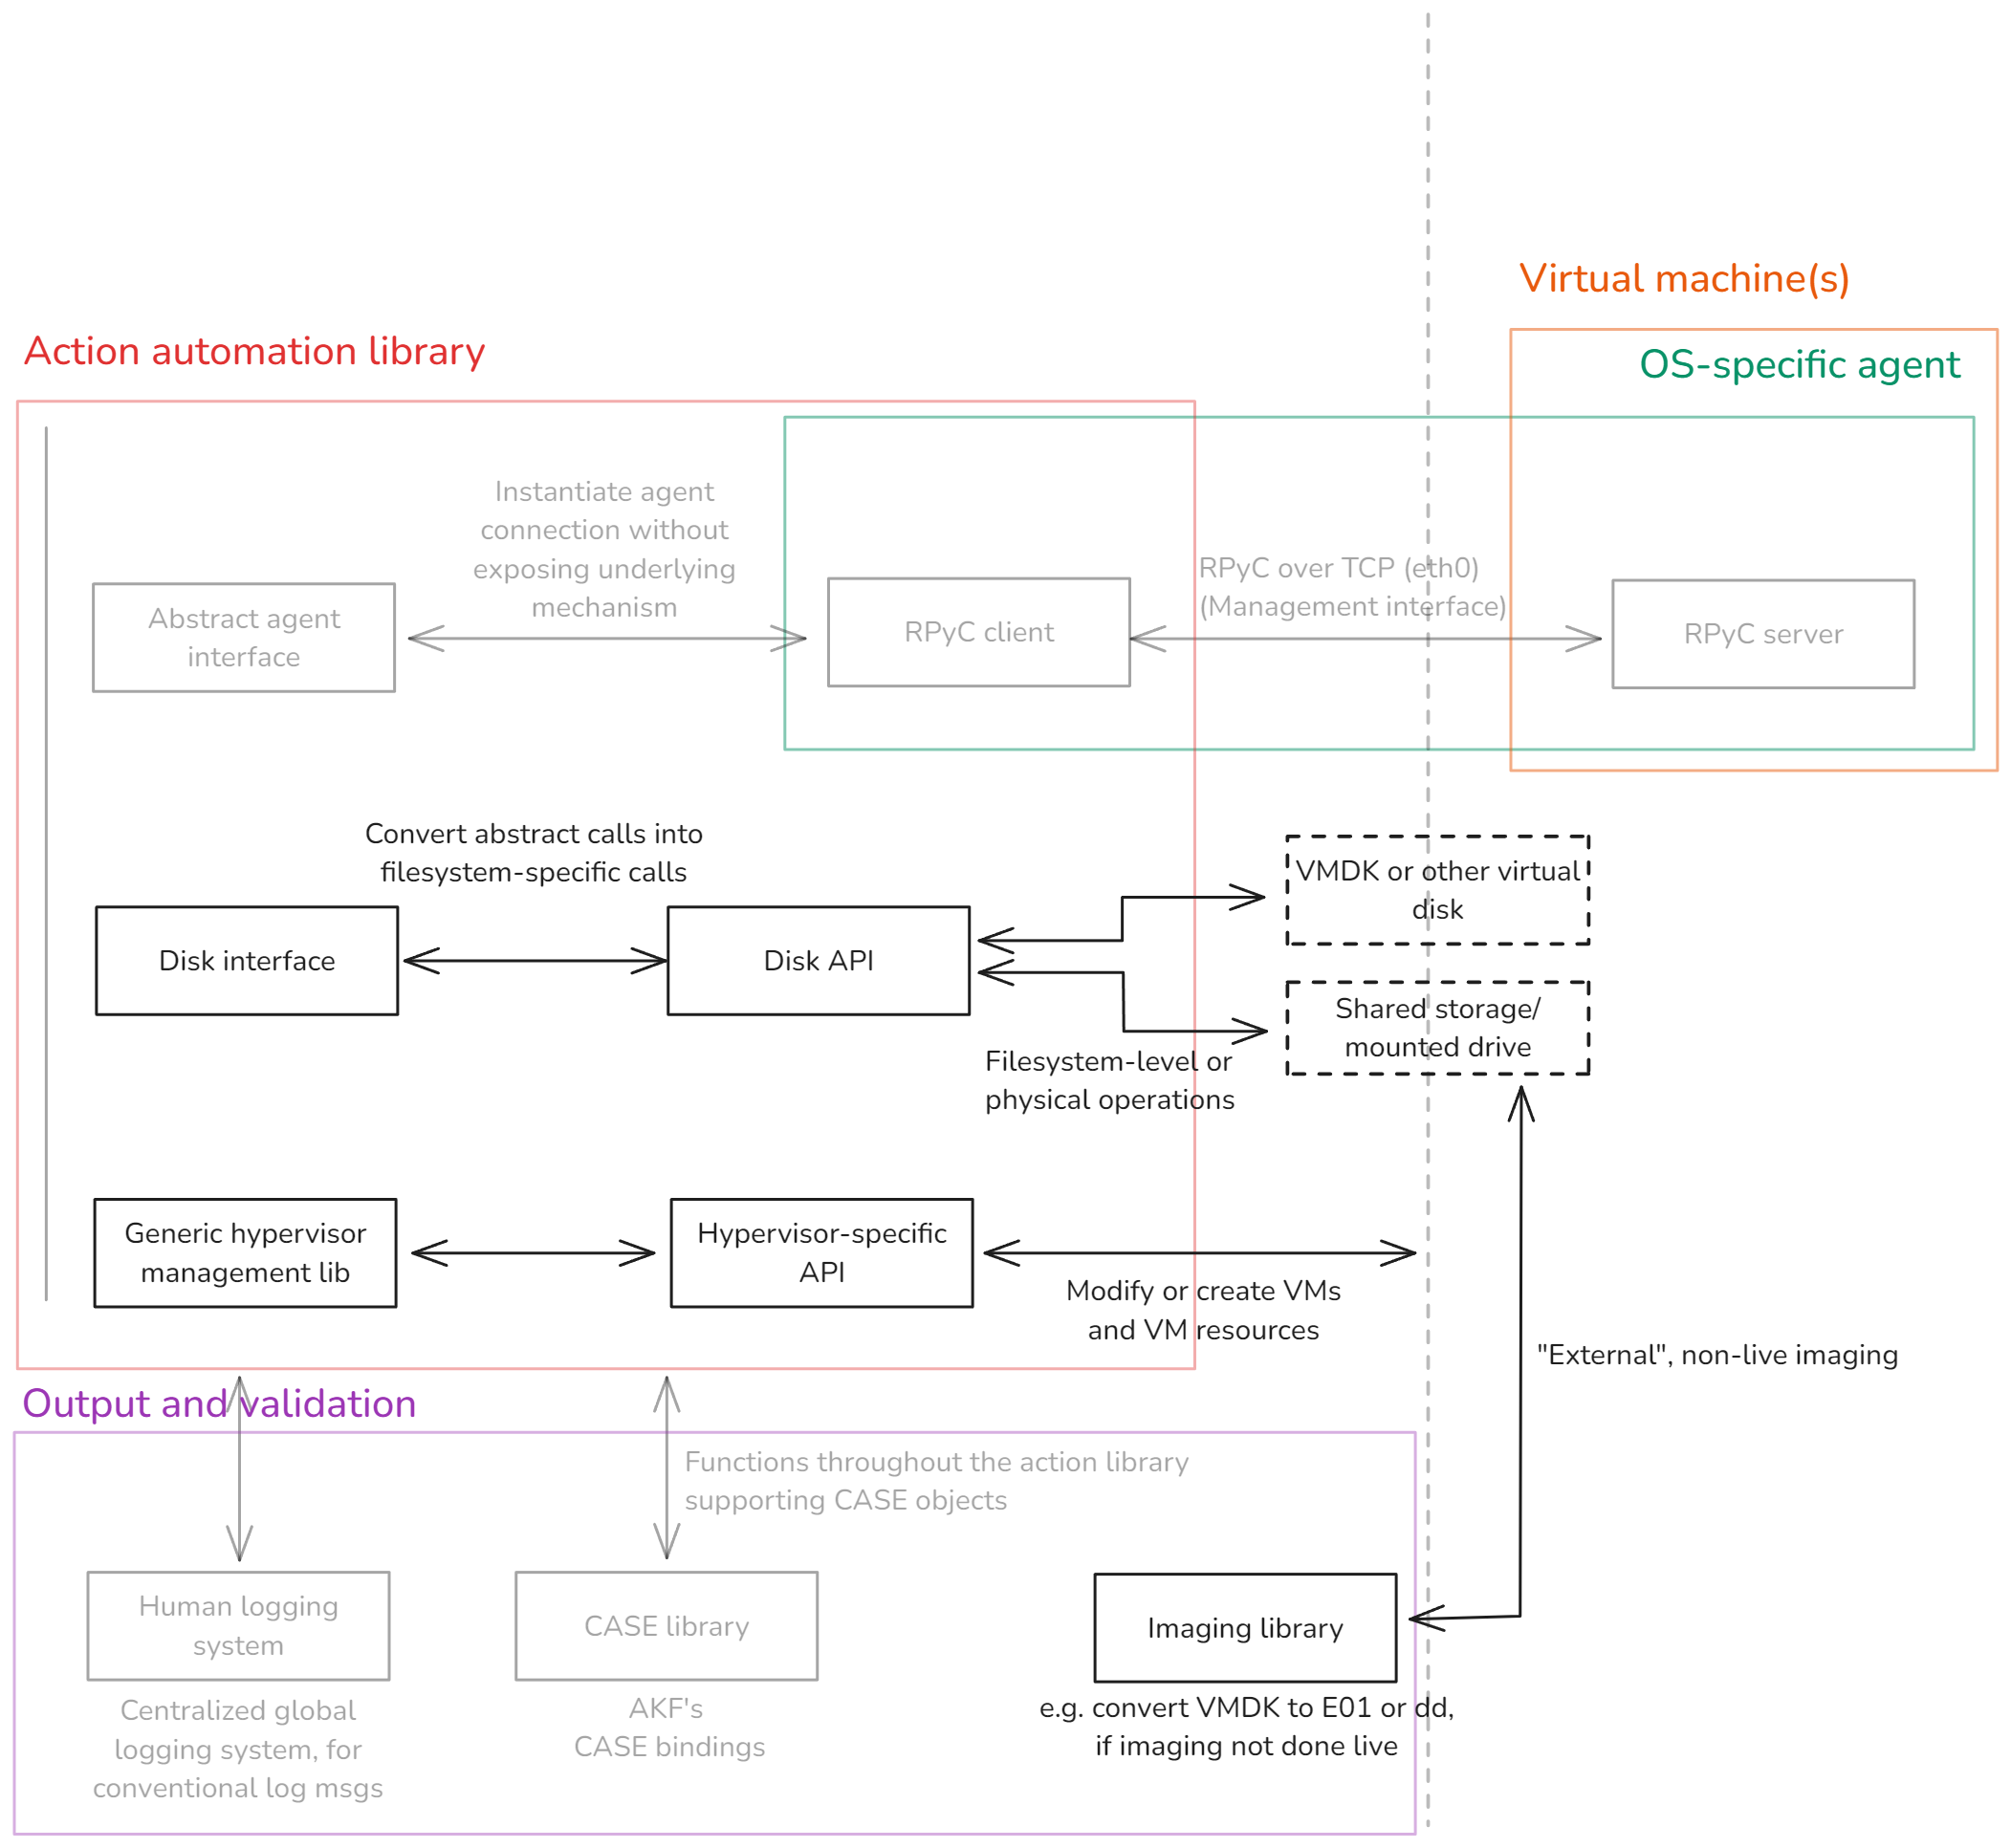
\includegraphics[width=1\linewidth]{action-physical.png}
\caption{Abridged submodule diagram for agent-based artifact
creation}\label{fig:action-physical}
\end{figure}

First, AKF does not currently support mounting and writing to arbitrary
filesystems or disk image formats, though this could be implemented
using external image mounting software with the assistance of
filesystem-independent libraries such as PyFilesystem
\cite{PyFilesystemPyfilesystem22025}. However, AKF allows users to
construct new ISO files from an existing host directory using the
\passthrough{\lstinline!pycdlib!} library
\cite{lalancetteClalancettePycdlib2025}. These ISOs can be used as
standalone artifacts (for example, presenting them to students as disk
images of removable drives) or as removable storage on a running virtual
machine. Mounting these ISOs, as well as setting up a shared network
folder between the host and guest machines, are the simplest means
through which scenario developers can transfer files onto a running
virtual machine.

Second, AKF also trivially ``supports'' filesystem-independent direct
editing. Python allows users to open files in binary mode, at which
point the user can call \passthrough{\lstinline!seek()!} on the file
pointer to advance the pointer to a specific offset in the file. The
user can then call \passthrough{\lstinline!write()!} to overwrite an
arbitrary number of bytes at that position, achieving the same outcome
as many other synthesizers that implement range and offset-based disk
image editing.

Although writing to arbitrary positions is not always viable for
correctly placing artifacts on a disk image, it is still a valid
approach when the underlying filesystem has already been analyzed and
the exact offsets and ranges to write are known. This may be the
approach used by EviPlant \cite{scanlonEviPlantEfficientDigital2017}
to construct and leverage its evidence packages for students; because
filesystem analysis is costly and requires additional libraries not
needed for offset-based editing, it is easier to perform this analysis
at construction time and distribute the offsets to which data must be
written to base images.

However, the filesystem may not have been analyzed ahead of time such
that the exact offsets and data needed to place a file on disk are
known. This brings us to filesystem-aware direct editing, in which AKF
makes significant improvements.

ForGe implements its physical artifact generation by implementing NTFS
and FAT32 data structures in Python, allowing it to create a fully
virtual representation of these filesystems (with the assistance of a
custom C program). This virtualized filesystem provides ForGe with the
information necessary to efficiently insert data into known slack and
unallocated space while maintaining filesystem consistency. While
extremely powerful (and implements a valuable feature not found in any
other synthesizer to date), it is inflexible in two specific aspects:

\begin{itemize}
\tightlist
\item
  ForGe does not provide a generic interface for the filesystems it
  supports. Although the NTFS and FAT32 wrappers provide the same
  methods with the same signatures, this is not strictly enforced by a
  parent class. The lack of a generic interface means that the
  functionality supported across all filesystems is unclear, as is the
  functionality that must be implemented for new filesystems to be
  compatible with ForGe.
\item
  ForGe lacks a ``frontend'' to support arbitrary disk types, regardless
  of the underlying filesystem. ForGe does not support multi-partition
  disks or common non-raw disk formats such as VHD, VMDK, or VDI.
\end{itemize}

Read-only libraries addressing these two issues have been in development
since the introduction of ForGe but have not been integrated into other
synthesizers to achieve the same write capabilities as ForGe. One such
library is \passthrough{\lstinline!libtsk!} (also known as The Sleuth
Kit), the C++ library that powers the open-source digital forensics
software Autopsy \cite{SleuthkitSleuthkit2025}.
\passthrough{\lstinline!libtsk!} allows users to navigate and analyze
the low-level contents of a variety of filesystems, including
filesystem-specific attributes and the sequence of disk clusters that
form a file. \passthrough{\lstinline!libtsk!} supports a large variety
of filesystems through a filesystem-agnostic interface, including the
FAT family of filesystems, the ext family, NTFS, and a variety of other
filesystems. ~It also supports various volume systems for
multi-partition disks, such as GPT and MBR, as well as several
filesystem containers and images.

Python bindings for \passthrough{\lstinline!libtsk!} have existed for at
least 15 years, with the most commonly used library being the
automatically generated \passthrough{\lstinline!pytsk!}
\cite{Py4n6Pytsk2025}. However, \passthrough{\lstinline!pytsk!} has
relatively limited Python documentation and adoption, in addition to
inheriting various known issues and limitations in
\passthrough{\lstinline!libtsk!}, such as support for niche filesystems
and partitioning formats. Many of these gaps were gradually covered as
part of the \passthrough{\lstinline!libyal!} project, a collection of
DFIR libraries developed by various contributors - most notably Joachim
Metz from Google \cite{LibyalLibyal2025}. The
\passthrough{\lstinline!libyal!} project includes individual libraries
for analyzing formats not supported by \passthrough{\lstinline!libtsk!},
such as the QCOW disk image format used by QEMU, the Apple File System
used by modern Apple devices, and more.

These libraries eventually led to the development of
\passthrough{\lstinline!dfvfs!}, or the Digital Forensics File System, a
Python library that leverages \passthrough{\lstinline!libtsk!} and
multiple libraries from the \passthrough{\lstinline!libyal!} project to
provide a generic interface for analyzing a variety of disk image
formats and filesystems \cite{Log2timelineDfvfs2025}. (The project
is derived from Plaso and Google Rapid Response, two open-source DFIR
tools used in various contexts.) Much like
\passthrough{\lstinline!libtsk!}, it exposes a variety of low-level
filesystem concepts common across multiple filesystems, such as the
metadata and individual segments comprising a file at a known path on
the filesystem. This low-level detail makes it extremely powerful in
performing filesystem-aware direct editing, especially because of its
focus on exposing this detail through a consistent Python interface.

AKF uses \passthrough{\lstinline!dfvfs!} to locate the clusters of a
file at a known path in a filesystem, which can then be used to identify
the start of slack space within the file's clusters (as well as
unallocated space in the filesystem). By adding the physical offset of
the cluster within the filesystem to the offset of the filesystem's
partition in the disk image, AKF can write to the exact location of a
file's slack space using the offset-based method described earlier. This
achieves feature parity with ForGe, completely delegating filesystem and
image-specific details to \passthrough{\lstinline!dfvfs!} and allowing
for a filesystem-independent method for locating slack space.

More generally, this technique provides a deterministic method for
inserting data within the slack space of a filesystem, simulating the
deallocation of a file and its partial replacement with a known file.
However, this does not fully simulate the process of deleting a file
through a running operating system and having a new file replace the
deallocated clusters; naturally, this does not generate OS-specific
artifacts associated with deleting and creating files and fails to
generate the filesystem artifacts that could exist with the original
file (such as the ``deleted'' file's name in the NTFS master file
table). Future work in the field could address this gap by combining
\passthrough{\lstinline!dfvfs!} with additional technologies to improve
the accuracy of physical techniques.

It should be noted that this technique does not work on filesystems with
full disk encryption enabled, as is the default on Windows systems
beginning with the Windows 11 24H2 update. Additionally, this technique
has only been verified to work on raw disk image formats. From limited
testing, the offsets of partitions and files on compacted formats such
as VHD are reported by \passthrough{\lstinline!dfvfs!} as if the
partition were not compact, which makes it difficult to correctly
determine the physical offset of a file on a VHD image. Additional
research is needed to develop a reliable method for performing
filesystem-aware physical artifact generation on such disk image
formats.
